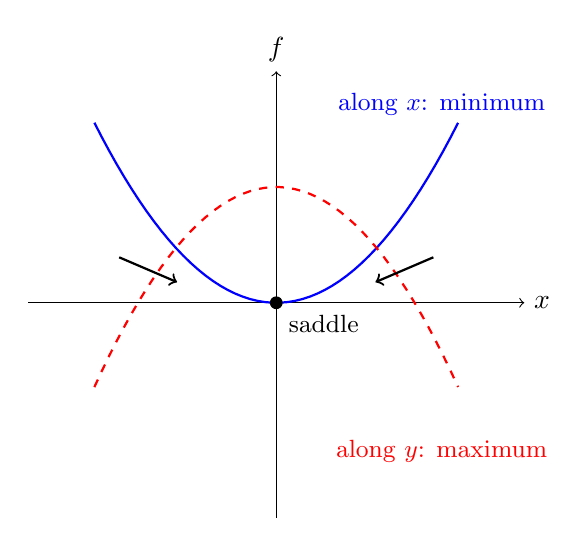
\begin{tikzpicture}[scale=1.05]
% saddle z = x^2 - y^2 rendered as two directional sections
\draw[->] (-3,0)--(3,0) node[right]{$x$};
\draw[->] (0,-2.6)--(0,2.8) node[above]{$f$};
\draw[thick,blue,domain=-2.2:2.2,samples=50] plot (\x,{0.45*\x*\x});
\node[blue] at (2.0,2.4) {\small along $x$: minimum};
\begin{scope}[yshift=-0.4cm]
\draw[thick,red,domain=-2.2:2.2,samples=50,dashed] plot (\x,{-0.5*\x*\x+1.8});
\node[red] at (2.0,-1.4) {\small along $y$: maximum};
\end{scope}
\fill (0,0) circle (2.2pt) node[below right=1pt]{\small saddle};
\draw[->,thick] (-1.9,0.55) -- (-1.2,0.25);
\draw[->,thick] (1.9,0.55) -- (1.2,0.25);
\end{tikzpicture}
